%!Tex Root = ../Tutorat6.tex
% ./Packete.tex
% ./Design.tex
% ./Deklarationen.tex
% ./Aufgabe2.tex
% ./Aufgabe3.tex
% ./Bonus.tex

\section{Task 1}

\setcounter{task}{1}

\begin{frame}[allowframebreaks]{Task 1}{}
  \begin{tasknoinc}
    \centering
    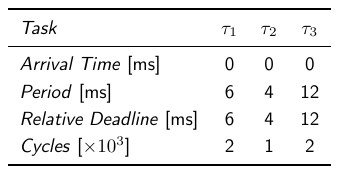
\includegraphics[width=0.4\textwidth]{./figures/task1_tasks.png}

    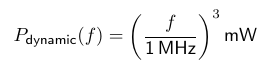
\includegraphics[width=0.4\textwidth]{./figures/task1_power.png}
  \end{tasknoinc}
  \begin{solutionnoinc}
    \begin{itemize}
      \item The execution times $C_i$ of tasks $\tau_i$ are: $C_1 = \frac{1 \cdot 10^3 Cyles}{1 \cdot 10^6 \frac{Cycles}{s}} =  2 ms$, $C_2 = \frac{1 \cdot 10^3 Cyles}{1 \cdot 10^6 \frac{Cycles}{s}} =  1 ms$, and $C_3 = \frac{1 \cdot 10^3 Cyles}{1 \cdot 10^6 \frac{Cycles}{s}}  = 2 ms$ ($T = \frac{N}{f}$).
      \item Applying EDF schedule, the processor is busy in $[0 ms, 9 ms]$
      \item constant input power: $P_{in} = 0.5\mu J$
      \item We use $1MHz$ for processing tasks, leading to $P_{\text{dynamic}}(1MHz) = 1mW$
      \item This means we consume $1mW \cdot 1ms = 1\mu J$ per milisecond.
      \item Since all our tasks take a multiple of 1ms, we know that while processing tasks, our battery empties with $0.5\mu J/ms - 1\mu J/ms = -0.5\mu J/ms$
      %and $P_{\text {dynamic }}(1MHz)=\left(\frac{1MHz}{1 \mathrm{MHz}}\right)^3 \mathrm{~mW} = 1 \cdot 10^{-3} W$ $\Rightarrow$ $0.5 \cdot 10^{-3}W - 1 \cdot 10^{-3}W = -0.5 mW$ and $-0.5 \cdot 10^{-3}W \cdot 2 \cdot 10^{-3}s = -1 \cdot 10^{-6}J = -1\mu J$ lost in first $2ms$ of the schedule.
    \end{itemize}
  \end{solutionnoinc}
  \begin{solutionnoinc}
    \centering
    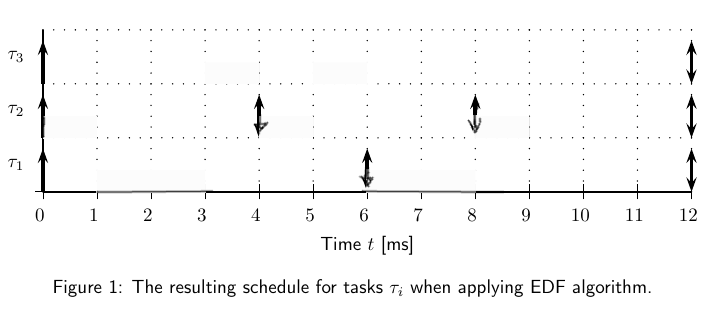
\includegraphics[height=0.6\paperheight]{./figures/task1_schedule_empty.png}
  \end{solutionnoinc}
  \begin{solutionnoinc}
    \centering
    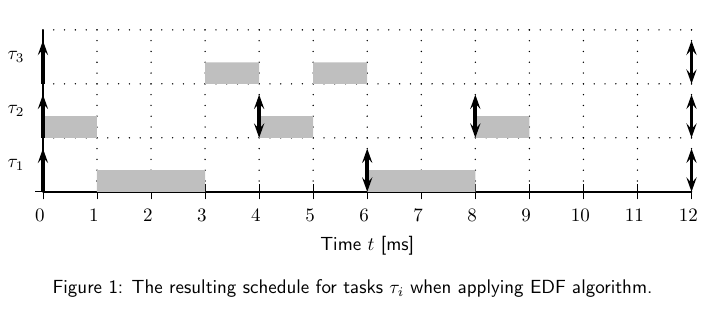
\includegraphics[height=0.6\paperheight]{./figures/task1_schedule.png}
  \end{solutionnoinc}
  \begin{solution}
    \centering
    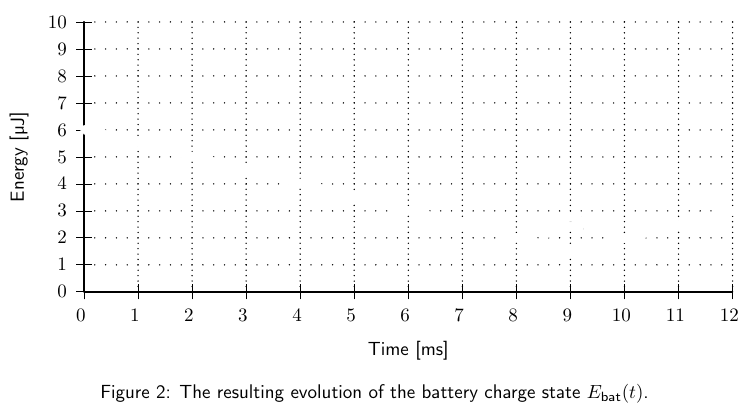
\includegraphics[height=0.6\paperheight]{./figures/task1_energy_empty.png}
  \end{solution}
  \begin{solution}
    \centering
    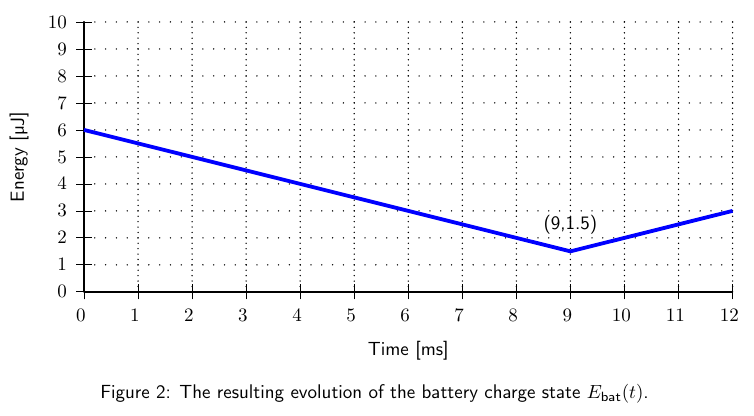
\includegraphics[height=0.6\paperheight]{./figures/task1_energy.png}
  \end{solution}
  \framebreak
  \begin{tasknoinc}
    \begin{itemize}
      \item To maximize the energy stored in the battery at the end of each hyper-period ($12 ms$), all tasks $ \tau_i$ have to be executed at the same frequency and this frequency leads to a utilization of $1.0$
    \end{itemize}
  \end{tasknoinc}
  \framebreak
  \begin{requirementsnoinc}
    \begin{itemize}
      \item \alert{processor utilization} $\displaystyle U_p = \sum_{i=1}^n \frac{C_i}{T_i}$
      \item the given power consumption $P_{dynamic}(f)$ is a \alert{strictly convex} function of the frequency $f$
      \item The EDF scheduling algorithm where deadlines of tasks equal their periods guarantees a feasible schedule as long as the utilization of the processor is $U \le 1.0$
        \begin{itemize}
          \item this schedulability test is \alert{necessary} and \alert{sufficient}, i.e. if one reaches a utilization of exactly $U = 1.0$, then it has to be schedulable
        \end{itemize}
    \end{itemize}
  \end{requirementsnoinc}
  \begin{requirementsnoinc}
    \centering
    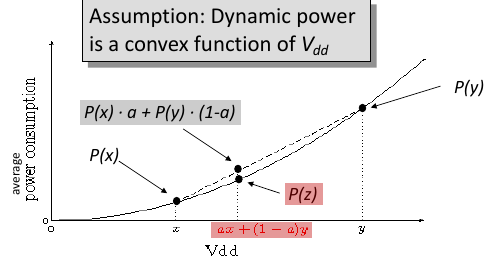
\includegraphics[width=0.5\textwidth]{./figures/task2_power_convex.png}
    \begin{itemize}
        \item The same argument applies if the power is a convex function of the \alert{frequency}!
    \end{itemize}
  \end{requirementsnoinc}
  \begin{solutionnoinc}
    \begin{itemize}
      \item The execution of all tasks with a constant frequency allows for a schedule where the utilization satisfies $U = 1.0$, i.e., the processor is constantly busy
        \begin{itemize}
          \item determine right frequency by looking at schedule: $\frac{9}{12} = 0.75$
          \item determine right frequency by calculation:
            \begin{itemize}
              \item $1 = \frac{\frac{2 kCycles}{f}}{6ms} + \frac{\frac{1 kCycles}{f}}{4ms}  + \frac{\frac{2 kCycles}{f}}{12ms} = \frac{\frac{4 kCycles + 3 kCycles + 2 kCycles}{f}}{12ms} \Leftrightarrow f = \frac{9 \cdot 10^3 Cycles}{12 \cdot 10^{-3} s} = 0.75 \cdot 10^{3 + 3} \cdot \frac{1}{s}  = 0.75MHz$
            \end{itemize}
        \end{itemize}
      \item the optimality of processing at a constant frequency during the whole time follows the same argumentation used to derive the optimal Dynamic Voltage and Frequency Scaling (DVFS).
      \begin{itemize}
        \item Due to the strict convexity of the power consumption $P_{dynamic}(f)$ the increase in the average power consumption of the higher frequency task always dominates the savings in the average power consumption of the lower frequency task execution.
      \end{itemize}
    \end{itemize}
  \end{solutionnoinc}
  \begin{solutionnoinc}
    \small
    \begin{itemize}
      \item the above conditions (constant frequency during execution, processor executing all the time) lead to a schedule, where the maximum frequency of task execution can not be further reduced as the whole time interval where tasks can be executed is filled with execution and all tasks are executed with the same frequency.
    \end{itemize}
  \end{solutionnoinc}
\end{frame}
